

\documentclass[11pt]{article}
% motion_header.tex
% include this before the \begin{document} part of your LaTeX source file
%
\usepackage{fourier,ifthen,xspace,amsmath,array}
\usepackage[svgnames, dvipsnames]{xcolor}
\usepackage{graphicx}
\usepackage{siunitx}
\usepackage{xkeyval,calc,moreverb}
\usepackage[breakable,skins]{tcolorbox}
\usepackage{booktabs}
\usepackage{paralist}

% booleans we need
\newboolean{bw}
\setboolean{bw}{false}
\newboolean{solutions}

% counters

\newcounter{problemctr}

% colors

\definecolor{probLineColor}{rgb}{0.2,0.6,0.2}
\definecolor{probLabelColor}{rgb}{0,0,0} % 0.2,0.2,0.7}
\definecolor{probStatementColor}{rgb}{0,0,0}
\definecolor{solColor}{rgb}{0.2,0.6,0.2}

% lengths

\newlength{\probLineWidth} \setlength{\probLineWidth}{1.25pt}
\newlength{\solLineWidth} \setlength{\solLineWidth}{0.5pt}

% oops!
\setlength{\probLineWidth}{0pt}
\setlength{\solLineWidth}{0pt}

% commands

\newcommand{\probdir}{/Users/saeta/Documents/Courses/p24/motion/prob/}
\newcommand{\figdir}{/Users/saeta/Documents/Courses/p24/motion/figs/}
\renewcommand{\probdir}{}
\renewcommand{\figdir}{}
\newcommand{\prob}[2]{% arguments are chapter then problem
  \input{\probdir ch#1/#1P#2}
}

\newcommand{\fig}[2][2]{%
 \vspace*{-.1in}
  \begin{center}%
    \includegraphics[width=#1in]{\figdir#2}
  \end{center}%
}

\newcommand{\SolutionHead}{Solution:}
\newcommand{\theexercise}{}
\newcommand{\PNScolor}[1]{\ifthenelse{\boolean{bw}}{}{\color{#1}}}
\newcommand{\SOL}[1]{\ifthenelse{\equal{#1}{0}}%
  {
\let\solution=\comment
\let\endsolution=\endcomment
\setboolean{solutions}{false}
}%
{\setboolean{solutions}{true}%
\renewenvironment{solution}%
{\par\noindent{\color{solColor}\rule{\linewidth}{\solLineWidth}%
\ifthenelse{\equal{#1}{}}%
{}%
{\par\smallskip\noindent\textbf{\SolutionHead}}}}{}}
}


\newcommand{\val}[2]{\ensuremath{#1~\mathrm{#2}}\xspace}	% number plus unit
\newcommand{\pval}[2]{\ensuremath{\left(#1~\mathrm{#2}}\right)\xspace}
\newcommand{\hval}[2]{\ensuremath{#1$-$\mathrm{#2}}\xspace}
\newcommand{\dg}[1]{\ensuremath{#1^{\circ}}\xspace}
\newcommand{\half}{\ensuremath{\frac{1}{2}}\xspace}
\newcommand{\ux}{\ensuremath{\mathbf{\hat{x}}}\xspace}
\newcommand{\uy}{\ensuremath{\mathbf{\hat{y}}}\xspace}
\newcommand{\uz}{\ensuremath{\mathbf{\hat{z}}}\xspace}
\newcommand{\ur}{\ensuremath{\mathbf{\hat{r}}}\xspace}
\newcommand{\vv}{\ensuremath{v}\xspace}

\newcommand{\xaxis}{$x$ axis\xspace}
\newcommand{\yaxis}{$y$ axis\xspace}
\newcommand{\zaxis}{$z$ axis\xspace}
\newcommand{\xyplane}{$xy$ plane\xspace}
\newcommand{\xzplane}{$xz$ plane\xspace}
\newcommand{\DOT}{\ensuremath{\boldsymbol{\cdot}}}

\newcommand{\bo}{\ensuremath{\boldsymbol{\omega}}\xspace}
\newcommand{\bO}{\ensuremath{\boldsymbol{\Omega}}\xspace}
\newcommand{\VEC}[1]{\ensuremath{\mathbf{#1}}\xspace}
\newcommand{\AU}{\ensuremath{\mathrm{A.U.}}\xspace}
\newcommand{\DB}{\ensuremath{\mathrm{dB}}\xspace}
\newcommand{\degC}[1]{\ensuremath{#1^{\circ}\mathrm{C}}\xspace}


% environments
\newcommand{\problabel}{Problem}
\newenvironment{problem}[1][]%
{
  \begingroup\refstepcounter{problemctr}
  \ifthenelse{\boolean{solutions}}%
    {
      {\vspace*{-10pt}\noindent\PNScolor{probLineColor}%
        \rule[-5pt]{\linewidth}{\probLineWidth}}
    }{}
  \begin{list}{%
      \PNScolor{probLabelColor}\textbf{\problabel\theexercise}%
    }{%
      \setlength{\labelsep}{0pt}%
      \setlength{\leftmargin}{0in}%
      \setlength{\labelwidth}{0pt}%
      \setlength{\listparindent}{0pt}
    }%
    \PNScolor{probStatementColor}%
	\item%
	\ifthenelse{\equal{#1}{}}%
      {}%
      {\textbf{ -- #1}}%
      \quad
}%
{%
  \end{list}\endgroup%
  \PNScolor{black}%
}

\newcommand{\PAGE}[2]{#1-#2\xspace}

\newenvironment{solution}{}{}
\newenvironment{question}{\renewcommand{\problabel}{Question}\begin{problem}}
{\end{problem}\renewcommand{\problabel}{Problem}}

\SOL{1} % show solution

\makeatletter
\newlength\rpLW
\newlength\rpRW
\newlength\rpgap
\newcommand{\rprcent}{0}
\newcommand{\rplcent}{0}
\define@key{rp}{lwidth}{\setlength{\rpLW}{#1}  \setlength{\rpRW}{\columnwidth-#1-\rpgap}}
\define@key{rp}{rwidth}{\setlength{\rpRW}{#1} \setlength{\rpLW}{\columnwidth-#1-\rpgap}}
 \define@key{rp}{lvert}{\def\LeftVerticalCode{#1}}
\define@key{rp}{rvert}{\def\RightVerticalCode{#1}}
\define@key{rp}{gap}{\setlength{\rpgap}{#1}}
\define@key{rp}{rcent}{\def\rprcent{#1}}
\define@key{rp}{lcent}{\def\rplcent{#1}}
\setkeys{rp}{rwidth=2in, lvert=c, rvert=t, gap=0.25in, rcent=0, lcent=0}
\makeatother

\newcommand\rp[3][]{%
  \setkeys{rp}{#1}
  \noindent \parbox[\LeftVerticalCode]{\rpLW}%
  {\ifthenelse{\equal{\rplcent}{0}}%
  {#2}%
  { \begin{center}#2\end{center} }%
  }%
  \hspace*{\rpgap}%
  \parbox[\RightVerticalCode]{\rpRW}%
  {\ifthenelse{\equal{0}{\rprcent}}%
  {#3}%
  {\begin{center} #3 \end{center}}}%
}

\newcommand{\DD}{\ensuremath{d}}		% differential d without leading space
\newcommand{\dd}{\ensuremath{\,\DD}}	% differential d

\newcommand{\deriv}[3][]{\ensuremath{%
	\ifthenelse{\equal{#1}{}}{\frac{\DD #2}{\DD #3}}
	{\frac{\DD^{#1} #2}{\DD #3^{#1}}}}}

\newcommand{\pd}[3][]{\ensuremath{%
	\ifthenelse{\equal{#1}{}}{\frac{\partial #2}{\partial #3}}
	{\partial #2 / \partial #3}}}

\newcommand{\so}{\ensuremath{\qquad\Longrightarrow\qquad}}
\newcommand{\uth}{\ensuremath{\boldsymbol{\hat{\theta}}}\xspace}
\newcommand{\eref}[2][]{%
	\ifthenelse{\equal{#1}{}}%
	{Eq.~(\ref{eq:#2})}%
	{Equation~(\ref{eq:#2})}\xspace}
\newcommand{\cross}{\ensuremath{\times}\xspace}
\newcommand{\into}{\ensuremath{\hat{\otimes}}}	% direction symbols
\newcommand{\outof}{\ensuremath{\hat{\odot}}}
\newcommand{\ds}{\displaystyle}

\newcommand{\xdd}{\ensuremath{\ddot{x}}\xspace}
\newcommand{\thdd}{\ensuremath{\ddot{\theta}}\xspace} % Download this file from physics.hmc.edu/motion/ page
\usepackage{tikz}

\usetikzlibrary{arrows,calc}
                	\tikzset{%
                         every picture/.style={>=stealth'},
                                        vel/.style={->,line width=2pt,color=DarkBlue},
                  force/.style={line width=1.5pt,color=blue,->},
                  coord/.style={color=green!40!black,|->},
                  accel/.style={->,line width=3pt,color=gray},
                  photon/.style={line width=1.5pt,color=DarkRed,decorate,decoration={snake,post length=0.1in}},
                  spring/.style={decorate,decoration={coil,aspect=0.3,segment length=2mm,amplitude=2mm}},
                  traj/.style={dashed, color=gray, line width=1pt}
                }
                
\usepackage{fullpage}
\setlength{\parskip}{6pt}
\setlength{\parindent}{0pt}
\usepackage[margin=1in]{geometry}
\usepackage{graphicx}
\usepackage{enumerate}
\usepackage{marvosym}
\usepackage{amssymb}
\usepackage{wasysym}
\usepackage{gensymb}
\usepackage{mathrsfs}
\usepackage{scrextend}
\usepackage{mathtools}
\usepackage{pgfplots}
\usepackage{xspace}
\usepackage[colorlinks]{hyperref}

\pgfplotsset{compat=1.15}
% --- style --- %
\renewcommand{\labelenumi}{{ (\alph{enumi})}}
\newcommand{\sand}{\quad \mbox{ and } \quad}
\newcommand{\be}{\begin{enumerate}[a) ]}
\newcommand{\ee}{\end{enumerate}}
\def\bal#1\eal{\begin{align*}#1\end{align*}}
\allowdisplaybreaks

% --- making \xi look less awful --- %
\DeclareSymbolFont{CMletters}{OML}{cmm}{m}{it}
\DeclareMathSymbol{\xi}{\mathord}{CMletters}{"18}

% --- math --- %
\newcommand{\Z}{\mathbb{Z}}
\newcommand{\R}{\mathbb{R}}
\newcommand{\C}{\mathbb{C}}
\newcommand{\Q}{\mathbb{Q}}


\newcommand{\Lt}[1]{\mathcal{L}\crb{#1}}
\newcommand{\ilt}[1]{\mathcal{L}^{-1}\crb{#1}}

\newcommand{\pn}[1]{\left( #1 \right)}
\newcommand{\sqb}[1]{\left[ #1 \right]}
\newcommand{\crb}[1]{\left\{ #1 \right\}}
\newcommand{\lra}[1]{\left\langle #1 \right\rangle}
\newcommand{\magn}[1]{\left\lVert #1 \right\rVert}

\def\multiset#1#2{\ensuremath{\left(\kern-.3em\left(\genfrac{}{}{0pt}{}{#1}{#2}\right)\kern-.3em\right)}}

\newcommand{\pdr}[2]{\frac{\partial #1}{\partial #2}}
\newcommand{\pdrr}[2]{\frac{\partial^2 #1}{\partial #2^2}}
\newcommand{\im}[1]{\text{im}\pn{#1}}
\newcommand{\m}[1]{\Z/#1\Z}


\DeclareMathOperator{\proj}{proj}
\newcommand{\vectorproj}[2][]{\proj_{\VEC{#1}}\VEC{#2}}

\newenvironment{amatrix}[1]{%
  \left(\begin{array}{@{}*{#1}{c}|c@{}}
}{%
  \end{array}\right)
}

\makeatletter
\renewcommand*\env@matrix[1][*\c@MaxMatrixCols c]{%
  \hskip -\arraycolsep
  \let\@ifnextchar\new@ifnextchar
  \array{#1}}
\makeatother

\newcommand{\spn}[1]{\text{span}\pn{#1}}

\newcommand*\Heq{\ensuremath{\overset{\kern2pt H}{=}}}

\newcommand{\distil}{\sqrt{1-v^2/c^2}}
\newcommand{\distilf}[1]{\sqrt{1-(#1)^2}}
\newcommand{\lorentz}{\frac{1}{\distil}}
\newcommand{\lorentzf}[1]{\frac{1}{\sqrt{1-(#1)^2}}}


\begin{document}

\noindent{\large Problem Set 12, 10 December 2018\hfill Name: \underline{\hspace{3cm}} ,  Section: \underline{\hspace{5mm}} }
\vspace*{0.25in}



\begin{problem}[Townsend (P1.19)]
Express the complex number $z_1 = (\sqrt{3} + i)/2$ in the form $re^{i\phi}$. What about 
$z_2 = (1 + \sqrt{3}i)/2$? If these complex numbers are the probability amplitudes for photons to be detected, what is the
probability in each case?
\end{problem}


% Your solution starts here %%%%%%%%%%%%%%%%%%%%%%%%%%%%%%%%%%%%%%%%%%%%%%%%%%
\textbf{Solution:}\\

\clearpage
% Your solution ends here %%%%%%%%%%%%%%%%%%%%%%%%%%%%%%%%%%%%%%%%%%%%%%%%%%

\begin{problem}[Townsend (P1.24)]
\be
\item Show that the probability of a photon of wavelength $\lambda$ being reflected from a thin layer of
glass of thickness $d$ at normal incidence is given by
\[	
	P = 0.16 \sin^2(2\pi d/\lambda')
\]
where $\lambda'$ is the wavelength of light in glass, i.e., 
$\lambda' = \lambda/n$, where $n$ is the index of refraction
in glass. \textit{Note}: In this calculation assume that the magnitude of the amplitude for reflection
from the top or the bottom surface of the glass is 0.2 and that there is an additional phase
change of $\pi$ in the reflection from the top surface. Also assume that amplitudes that arise
from multiple reflections between the top and bottom surfaces of the glass can be neglected in
your calculation. Given the result of Problem 1.23, it is okay to approximate the magnitude
of the amplitude for transmission as one. \textit{Hint}: What extra distance does light travel in being
reflected from the bottom surface relative to the top surface?
\item In \textit{QED: The Strange Theory of Light and Matter} Feynman states that as the thickness of a
thin layer of glass increases from zero thickness, the probability of reflection first reaches a
value of 0.16 when the thickness of the layer of glass is 5 millionths of an inch. What index
of refraction is being assumed? Take the wavelength of the light in air to be the same as you
determined in Problem 1.22, i.e. $\lambda = \val{706}{nm}$.
\item What is the minimum value of $d$ necessary to produce zero reflection?
\ee
\end{problem}


% Your solution starts here %%%%%%%%%%%%%%%%%%%%%%%%%%%%%%%%%%%%%%%%%%%%%%%%%%
\textbf{Solution:}\\

\clearpage
% Your solution ends here %%%%%%%%%%%%%%%%%%%%%%%%%%%%%%%%%%%%%%%%%%%%%%%%%%

\begin{problem}[Townsend (P1.25)*]
Suppose that a thin film of acetone (index of refraction $n = 1.25$) of thickness $d$ is coating a thick
plate of glass (index of refraction $=$ 1.50). Take the magnitude of the amplitude for reflection of a
photon from the top or the bottom surface of the acetone at normal incidence to be $r$ and assume
that there is an additional phase change of $\pi$ in the reflection from the top and the bottom surface
of the acetone, since at each of these surfaces light is passing from a medium with a lower index
of refraction to one with a higher index of refraction. Calculate the probability that a photon of
wavelength $\lambda$ is reflected. Assume that amplitudes that involve multiple reflections at the bottom
surface of the film can be neglected in your calculation. Express your answer in terms $\lambda$ and $r$ as
well as the thickness $d$ and the index of refraction $n$ of the acetone. What is the minimum thickness
of the coating necessary to produce zero reflection? \textit{Note}: For the air?acetone and acetone?glass
surfaces $r \approx 0.1$.
\end{problem}


% Your solution starts here %%%%%%%%%%%%%%%%%%%%%%%%%%%%%%%%%%%%%%%%%%%%%%%%%%
\textbf{Solution:}\\

\clearpage
% Your solution ends here %%%%%%%%%%%%%%%%%%%%%%%%%%%%%%%%%%%%%%%%%%%%%%%%%%

\begin{problem}[Townsend (P1.26)]
Assume that the first beam splitter at A in the Mach-Zehnder interferometer (the figure below) is a ``third-silvered
mirror," that is, a mirror that reflects one-third the light and transmits two-thirds. The two
mirrors at B and C reflect 100 \% of the light, and the second beam splitter at D is a traditional half-silvered
mirror that reflects one-half the light and transmits one-half. The probability of detecting
a photon in either photomultiplier $PM_1$ or $PM_2$ varies with the position of the movable mirror, say
mirror B. Determine the maximum probability and the minimum probability of obtaining a count
in, say, $PM_1$. What is the visibility
\[
	V = \frac{P_{\text{max}} - P_{\text{min}}}{P_{\text{max}} + P_{\text{min}}}
\]	
of the interference fringes, where $P_{\text{max}}$ and $P_{\text{min}}$ are the maximum and minimum probabilities,
respectively, that a photon is counted by the detector, as the position of the movable mirror varies?
\textit{Note}: In the experiment of Aspect et al. described in Section 1.5 the visibility of the fringes is
$0.987 \pm 0.005$.
\begin{center}
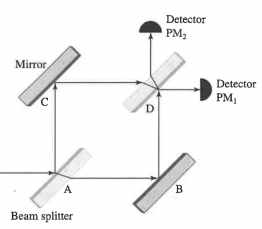
\includegraphics[scale=0.6]{prob4.png}
\end{center}
\end{problem}


% Your solution starts here %%%%%%%%%%%%%%%%%%%%%%%%%%%%%%%%%%%%%%%%%%%%%%%%%%
\textbf{Solution:}\\

\clearpage
% Your solution ends here %%%%%%%%%%%%%%%%%%%%%%%%%%%%%%%%%%%%%%%%%%%%%%%%%%

\begin{problem}[Townsend (P1.27)]
The figure below shows a Michelson interferometer with a movable mirror $M_1$, a fixed mirror $M_2$, and
a beam splitter $M_s$, which is a half-silvered mirror that transmits one-half the light and reflects
one-half the light incident upon it independent of the direction of the light. The source emits
monochromatic light of wavlength $\lambda$. There are two paths that light can follow from the source to
the detector, as indicated in the figure. Note that path 1 includes travel from the beam splitter
$M_s$ to the movable mirror $M_1$ and back to the beam splitter, while path 2 includes travel from the
beam splitter $M_s$ to the fixed mirror $M_2$ and back to the beam splitter. Assume the beam splitter
introduces a phase change of $\pi$ for light that follows path 1 from the source to the detector relative
to light that follows path 2 from the source to the detector. Also assume the mirrors $M_1$ and
$M_2$ reflect 100\% of the light incident upon them and the photodetector PM (a photomultiplier) is
100\% efficient as well.
\be
\item Use the principles of quantum mechanics to determine the probability that a photon entering
the interferometer is detected by the photodetector. Express your answer in terms of the
lengths $l_1$, $l_2$, and $\lambda$.
\item Find an expression for $l_1$ in terms of $l_2$ and $\lambda$ such that there is 100\% probability that the
photon is detected by the photodetector.
\item Suppose that the movable mirror is shifted upward by a distance $\lambda/6$ from the position(s)
that you determined in part (b). Find the probability that the photon is detected at the
photodetector in this case.
\ee
\begin{center}
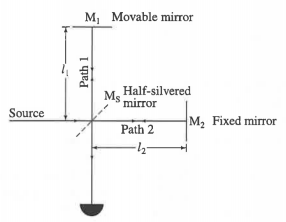
\includegraphics[scale=0.6]{prob5.png}
\end{center}
\end{problem}


% Your solution starts here %%%%%%%%%%%%%%%%%%%%%%%%%%%%%%%%%%%%%%%%%%%%%%%%%%
\textbf{Solution:}\\

\clearpage
% Your solution ends here %%%%%%%%%%%%%%%%%%%%%%%%%%%%%%%%%%%%%%%%%%%%%%%%%%

\begin{problem}[Townsend (P1.29) \P]
Suppose that the two very narrow slits (widths $\ll \lambda$) in the double-slit experiment are not the same
width and that the probability amplitude for a photon of wavelength $\lambda$ to strike a photomultiplier
centered at a particular point P in the detection plane that makes an angle $\theta$ with the horizontal
from one of the slits is larger by a factor of $\sqrt{2}$ than for the other slit. Determine the visibility
\[
	V = \frac{P_{\text{max}} - P_{\text{min}}}{P_{\text{max}} + P_{\text{min}}}
\]
of the interference fringes, where $P_{\text{max}}$ is the maximum probability and $P_{\text{min}}$ is the minimum probability that a photon is detected.
\end{problem}


% Your solution starts here %%%%%%%%%%%%%%%%%%%%%%%%%%%%%%%%%%%%%%%%%%%%%%%%%%
\textbf{Solution:}\\

\clearpage
% Your solution ends here %%%%%%%%%%%%%%%%%%%%%%%%%%%%%%%%%%%%%%%%%%%%%%%%%%

\begin{problem}[Townsend (P1.34) \P ]
Starting from first principles, show that the probability that a photon of wavelength $\lambda$ hits a
photomultiplier centered on a point P in the detection plane that makes an angle $\theta$ with the
horizontal for a grating composed of three very narrow slits each separated by a distance d is given
by
\[
	\text{Prob} = r^2\pn{1+4\cos\phi + 4\cos^2\phi}
\]	
where $r^2$ is the probability that the photon would strike the photomultiplier with a single slit open
and $\phi = kd\sin\theta = 2\pi d\sin\theta / \lambda$.
\end{problem}


% Your solution starts here %%%%%%%%%%%%%%%%%%%%%%%%%%%%%%%%%%%%%%%%%%%%%%%%%%
\textbf{Solution:}\\

\clearpage
% Your solution ends here %%%%%%%%%%%%%%%%%%%%%%%%%%%%%%%%%%%%%%%%%%%%%%%%%%

\end{document}